\chapter{Test\index{Test}}
\label{chp:test}
In the introduction in \chpref{chp:goal} we discussed our goals and mentioned we want to assess the usability of our process calculus for application in practice. In particular, we are interested in whether it's possible to achieve a speedup\index{Speedup} by using the developed process calculus for program parallelisation.

\section{Setup}
For the tests the ant system implementation from \chpref{chp:ant_system_implementation} is modified to give three different variants:
\begin{itemize}
  \item[$A_{seq}\colon$] An unparallelised version running everything sequentially
  \item[$A_{con}\colon$] A slightly changed, parallelised version using the process interpreter based on \textsf{Concurrent Haskell}
  \item[$A_{dis}\colon$] The unchanged, parallelised version using the process interpreter based on {Cloud Haskell}
\end{itemize}

As input for the ant systems, we use a set of 10 instances from the TSPLIB\footnote{\url{http://www.iwr.uni-heidelberg.de/groups/comopt/software/TSPLIB95/tsp/}}, a collection of instances of the travelling salesman problem\index{Travelling Salesman Problem} that have to be solved to optimality. The instances we're using are: \texttt{bays29}, \texttt{berlin52}, \texttt{st70}, \texttt{pr76}, \texttt{gr96}, \texttt{eil101}, \texttt{pr107}, \texttt{pr124}, \texttt{bier127} and \texttt{ch130}. The number included in the instance names give information about their size, i.e. the number of nodes in the graph described by the instance.

We configure the ant systems using parameters based on suggestions given in \cite{Dorigo:2004:ACO:975277}: we use $n$ ants for a graph of size $n$, $100$ iterations, $\tau_0 = 2$, $\alpha = 2$, $\beta = 5$ and $\rho = 0.1$.

Since $A_{seq}$, $A_{con}$ and $A_{dis}$ are implementations of the same meta-heuristic and only differ in the way they are parallelised, we expect to obtain approximate solutions of similar quality for the selected instances from all three variants. In fact, we're not interested in the proposed solutions but in the necessary time to obtain them. We use the runtime of $A_{seq}$ as a reference an compare the runtimes of $A_{con}$ and $A_{dis}$ against it.

The test runs to assess what speedup we can reach using $A_{con}$ and local parallelisation, compared to $A_{seq}$, are carried out on an $\text{Intel}^{\textregistered}$ $\text{Core}^{\texttrademark}$ i7-3770 CPU @ 3.4GHz with 16GB RAM. We use \textsf{ghc} to compile the programs and the compiler flags \texttt{-O2} for $A_{seq}$ and \texttt{-threaded -O2} for $A_{con}$. We run $A_{con}$ with 1, 2, 3 and 4 cores active, respectively, using the \texttt{+RTS -N} option.

The tests to assess what speedup we can reach using $A_{dis}$ and parallelisation in a distributed system, compared to $A_{seq}$, are carried out using a set of $\text{Intel}^{\textregistered}$ $\text{Core}^{\texttrademark}$ i5-2400 CPUs @ 3.1GHz with 4GM RAM. We use \textsf{ghc} to compile the programs and the compiler flags \texttt{-O2} for $A_{seq}$ and \texttt{-threaded -O2} for $A_{dis}$. We run $A_{dis}$ with the dedicated master node on one computer and with 4, 8, 16 and 32 worker nodes connected, respectively. Note that, as the used CPUs have 4 physical cores, each of them can be used to run 4 worker nodes.

\section{Results and interpretation}
The runtime of $A_{con}$ varies with the number of used physical cores. When only one core is used, it shows a higher runtime than $A_{seq}$. This is not particularly surprising since in this case both $A_{seq}$ and $A_{con}$ only have one core available, but $A_{con}$ introduces a management overhead that comes with the parallel formulation of the ant system. This overhead gets bigger for problem instances with higher number of nodes in the graph since for a graph of size $n$, we have decided to use $n$ ants that all run in parallel.

However, as the number of physical cores is increased, $A_{con}$ can achieve a speedup compared to $A_{seq}$. When 4 physical cores are used, the speedup factor ranges between $1.2$ and $1.56$, depending on the size of the problem instance. Note that according to \textsc{Amdahl}'s law, the maximum achievable speedup factor is bound by the sequential fraction of the ant system that cannot be parallelised. This includes e.g. processes composed using \texttt{Sequence} or synchronisation operations that are hidden in the implementation of the process interpreter \texttt{runProcess}. Even an infinite number of physical cores would not yield any further speedup.

\begin{table}[h!]
  \centering
  \begin{tabular}{r|c||c|c|c|c|}
    \cline{2-6}
    & \multicolumn{1}{c||}{$A_{seq}$} & \multicolumn{4}{c|}{$A_{con}$} \\
    \hline
    \multicolumn{1}{|r||}{scenario} & & 1 core & 2 cores & 3 cores & 4 cores \\
    \hline
    \hline
    \multicolumn{1}{|r||}{\texttt{bays29}} & 0.45s & 0.511s & 0.424s & 0.379s & 0.375s \\
    \hline
    \multicolumn{1}{|r||}{\texttt{berlin52}} & 2.253s & 2.561s & 2.016s & 1.657s & 1.521s \\
    \hline
    \multicolumn{1}{|r||}{\texttt{st70}} & 5.292s & 6.484s & 4.911s & 3.894s & 3.416s \\
    \hline
    \multicolumn{1}{|r||}{\texttt{pr76}} & 6.4s & 8.546s & 6.142s & 4.867s & 4.236s \\
    \hline
    \multicolumn{1}{|r||}{\texttt{gr96}} & 12.855s & 20.767s & 13.703s & 9.881s & 8.209s \\
    \hline
    \multicolumn{1}{|r||}{\texttt{eil101}} & 15.126s & 25.893s & 16.682s & 11.949s & 9.773s \\
    \hline
    \multicolumn{1}{|r||}{\texttt{pr107}} & 16.244s & 26.738s & 16.482s & 11.817s & 10.521s \\
    \hline
    \multicolumn{1}{|r||}{\texttt{pr124}} & 26.277s & 50.024s & 30.203s & 22.587s & 18.33s \\
    \hline
    \multicolumn{1}{|r||}{\texttt{bier127}} & 28.468s & 54.311s & 33.37s & 24.948s & 20.225s \\
    \hline
    \multicolumn{1}{|r||}{\texttt{ch130}} & 32.039s & 61.328s & 37.042s & 27.866s & 22.909s \\
    \hline
  \end{tabular}
  \caption{Runtimes of $A_{seq}$ and $A_{con}$ for the selected instances and configuration.}
  \label{tbl:test1}
\end{table}
The runtimes measured in the test setup to asses the speedup of $A_{con}$ compared to $A_{seq}$ can be found in table \ref{tbl:test1}. Figure \ref{fig:test_local} shows a plot of the runtimes.

\begin{figure}[h!]
  \centering
  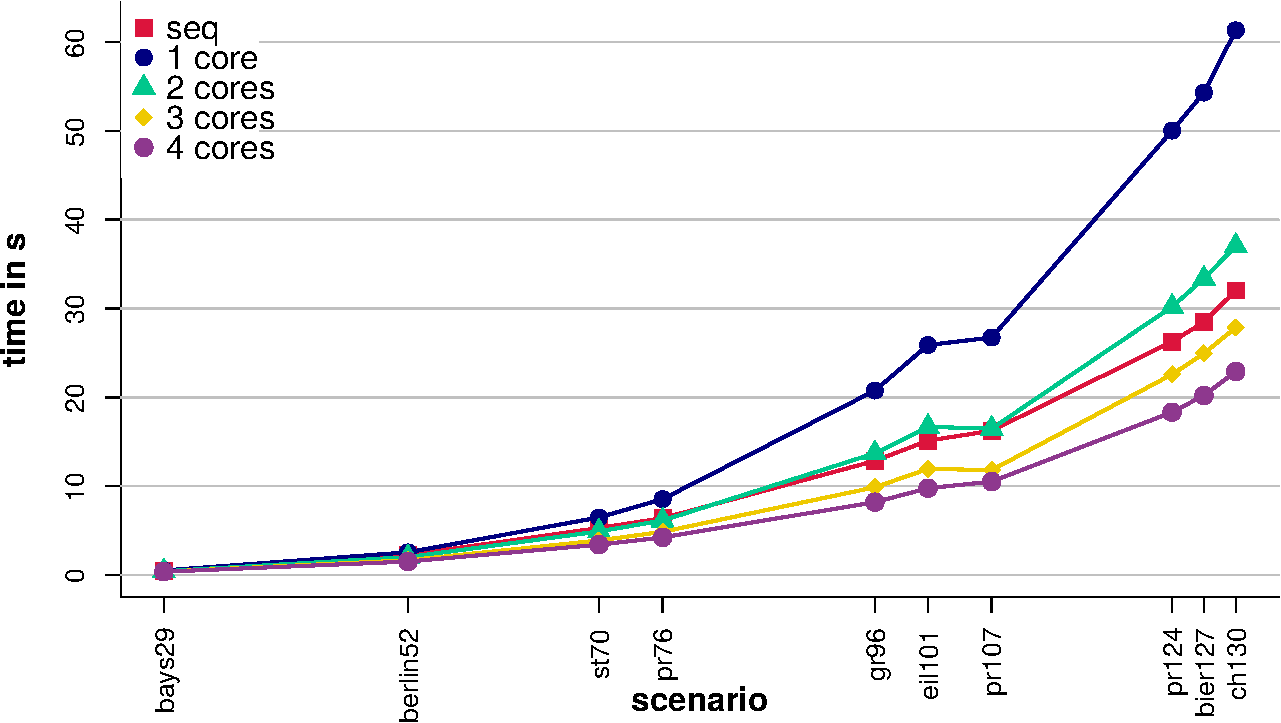
\includegraphics[width=\textwidth]{img/test_local.pdf}
  \caption{Plot of the runtimes of $A_{seq}$ and $A_{con}$.}
  \label{fig:test_local}
\end{figure}

The runtimes obtained in the test setup to asses the achievable speedup of $A_{dis}$ compared to $A_{seq}$ are shown in table \ref{tbl:test2} and are plotted in \figref{fig:test_distributed}. They show that $A_{dis}$ is unable to achieve a speedup. In fact, depending on the problem instance, $A_{dis}$ takes between ... and ... times as much time as $A_{seq}$ even with 32 worker nodes connected.

Several things may have to be taken into account to explain this. $A_{dis}$ involves a number of ant process that are executed in parallel, depending on the size of the problem instance. For each of the ant processes, the process interpreter \texttt{runProcess} has to contact the master node in order to obtain a worker node where the ant process can be spawned. The fact that \textsf{Cloud Haskell} used TCP communication for reliable delivery of messages, adds some overhead on top of the network communication that might be potentially slow anyway.

\begin{table}[h!]
  \centering
  \begin{tabular}{r|c||c|c|c|c|}
    \cline{2-6}
    & \multicolumn{1}{c||}{$A_{seq}$} & \multicolumn{4}{c|}{$A_{dis}$} \\
    \hline
    \multicolumn{1}{|r||}{scenario} & & 4 worker & 8 worker & 16 worker & 32 worker \\
    \hline
    \hline
    \multicolumn{1}{|r||}{\texttt{bays29}} & 0.893s & 59s & 36s & 30s & \\
    \hline
    \multicolumn{1}{|r||}{\texttt{berlin52}} & 4.552s & 191s & 117s & 91s & \\
    \hline
    \multicolumn{1}{|r||}{\texttt{st70}} & 10.493s & 363s & 255s & 193s & \\
    \hline
    \multicolumn{1}{|r||}{\texttt{pr76}} & 19.3s & 484s & 308s & 236s & \\
    \hline
    \multicolumn{1}{|r||}{\texttt{gr96}} & 25.595s & & 573 & & \\
    \hline
    \multicolumn{1}{|r||}{\texttt{eil101}} & & & & & \\
    \hline
    \multicolumn{1}{|r||}{\texttt{pr107}} & & & & & \\
    \hline
    \multicolumn{1}{|r||}{\texttt{pr124}} & & & & & \\
    \hline
    \multicolumn{1}{|r||}{\texttt{bier127}} & & & & & \\
    \hline
    \multicolumn{1}{|r||}{\texttt{ch130}} & & & & & \\
    \hline
  \end{tabular}
  \caption{Runtimes of $A_{seq}$ and $A_{dis}$ for the selected instances and configuration.}
  \label{tbl:test2}
\end{table}

Furthermore, for every remotely spawned process, a function closure has to be created, serialised and sent to a remote node over the network. In case of the ant system this includes redundant data: every ant receives a configuration that contains the problem instance. This problem instance never changes and could conceptually be cached on the worker nodes. However, at the moment the possibility to do so is not given, but leaves room for future improvements. Note that the problem of distributing data to parallel processes did not come up in the case of $A_{con}$: all processes execute on the same computer and have access to the same data structure that is kept in memory.

\begin{figure}[h!]
  \centering
  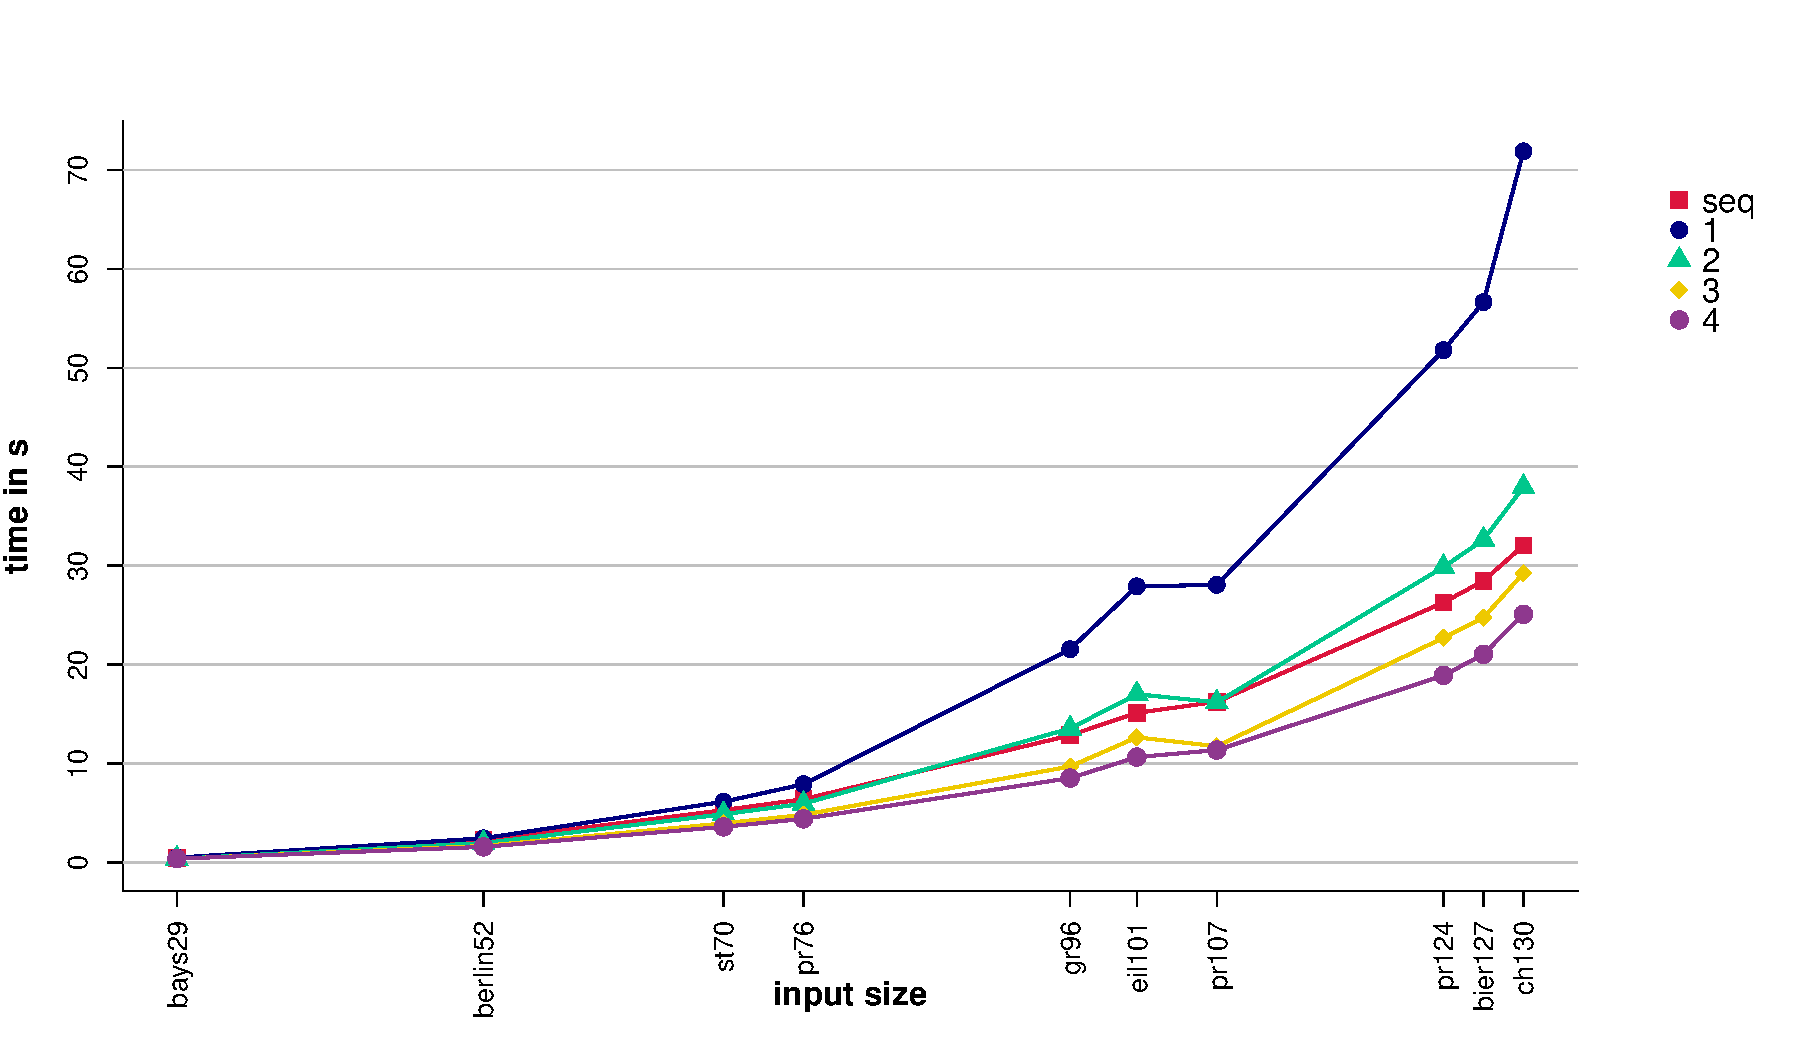
\includegraphics[width=\textwidth]{img/test_distributed_1.pdf}
  \caption{Plot of the runtimes of $A_{seq}$ and $A_{dis}.$}
  \label{fig:test_distributed}
\end{figure}